\section{Similarity Computation}
That is, given a pair of terms, our approach has basically two steps: We first
represent the semantic contexts for each of the terms, modeling a probability distribution over contexts and then we compare how similar
these two discrete probability distributions are by encoding them as vectors and computing the cosine between the vectors.


In this section, we give the similarity computation method between terms.
The terms mentioned in this paper involve two categories, namely the concept and the instance in our Probase. Hence, we could get three categories corresponding to the type of the term in the given pair, such as the concept-instance pair (e.g.,~$<Company,~Microsoft>$), the concept-concept~pair (e.g.,~$<Company,~Country>$) and the instance-instance~pair (e.g.,~$<Apple,~Microsoft>$). However, if the given pair of terms has a concept term, we can use the contexts of seeds as the context of the current concept. For example, given a concept term $Company$, the top 10 seed instances include \emph{Microsoft}, \emph{IBM}, \emph{Google}, \emph{Apple}, \emph{Dell}, \emph{Intel}, \emph{Sony}, \emph{Motorola}, \emph{HP} and \emph{Samsung}. Therefore, we can transform the issue of measuring semantic similarity between terms into that between instances.
Correspondingly, we can formalize the issue below. Given the pairwise terms $<e_{1}, e_{2}>$, we can get the semantic contexts, such as attribute-based and isA-based contexts for each instance as shown in Figure~\ref{fig:Information-structure-of-terms}. According to the collected semantic contexts, our current task is hence to evaluate the similarity between contexts. That is,
\begin{figure}[t]
%\makeatletter\def\@captype{figure}\makeatother
 \centerline{
 \includegraphics[width=0.5\textwidth]{Information-structure-of-terms.eps}}
\caption{Semantic contexts of given terms} \label{fig:Information-structure-of-terms}
\end{figure}
\begin{equation}
\begin{aligned}
sim(T(e_{1}), T(e_{2})) = f(sim(A_{e_{1}}, A_{e_{2}}), sim(\mathcal{I}_{e_{1}}, \mathcal{I}_{e_{2}}))
\label{eq:task1}
\end{aligned}
\end{equation}
\begin{displaymath}
{s.t.,
\begin{aligned}
sim(A_{e_{1}}, A_{e_{2}}) = cosine(A_{e_{1}}, A_{e_{2}})\\
sim(\mathcal{I}_{e_{1}}, \mathcal{I}_{e_{2}}) = cosine(\mathcal{I}_{e_{1}}, \mathcal{I}_{e_{2}})~~
\end{aligned}
}
\end{displaymath}
where $f()$ indicates the similarity evaluation function between contexts. In our approach, we use logistic regression to combine the attribute based similarity (e.g., $sim(A_{e_{1}}, A_{e_{2}})$) and the isA-based similarity (e.g., $sim(\mathcal{I}_{e_{1}}, \mathcal{I}_{e_{2}})$). 